\lab{Application}{Newton's Method, Julia Sets and Basins of Attraction}{Newton's Method}
\label{lab:NewtonsMethod}
\objective{Understand Newton's Method. Understand definition of basin of attraction.  Basic understanding of Julia Sets.}

One important technique in technical computing is Newton's method. The goal of Newton's method is to find $\overline{x}$ such that $f\left(\overline{x}\right) = 0$.
This method is especially important in optimization, where our goal is to find minima and maxima of functions.
Newton's method is an iterative method (much like eigenvalue finders: remember how those provably have to be iterative?).
Newton's method, in one dimension, is defined as follows:
\[
x_{n+1} = x_n - \frac{f(x_n)}{f'(x_n)}
\]

Essentially Newton's method approximates a function by its tangent line, and then uses the zero of the tangent line as the next guess for $x_n$.

\begin{figure}[h]
\centering
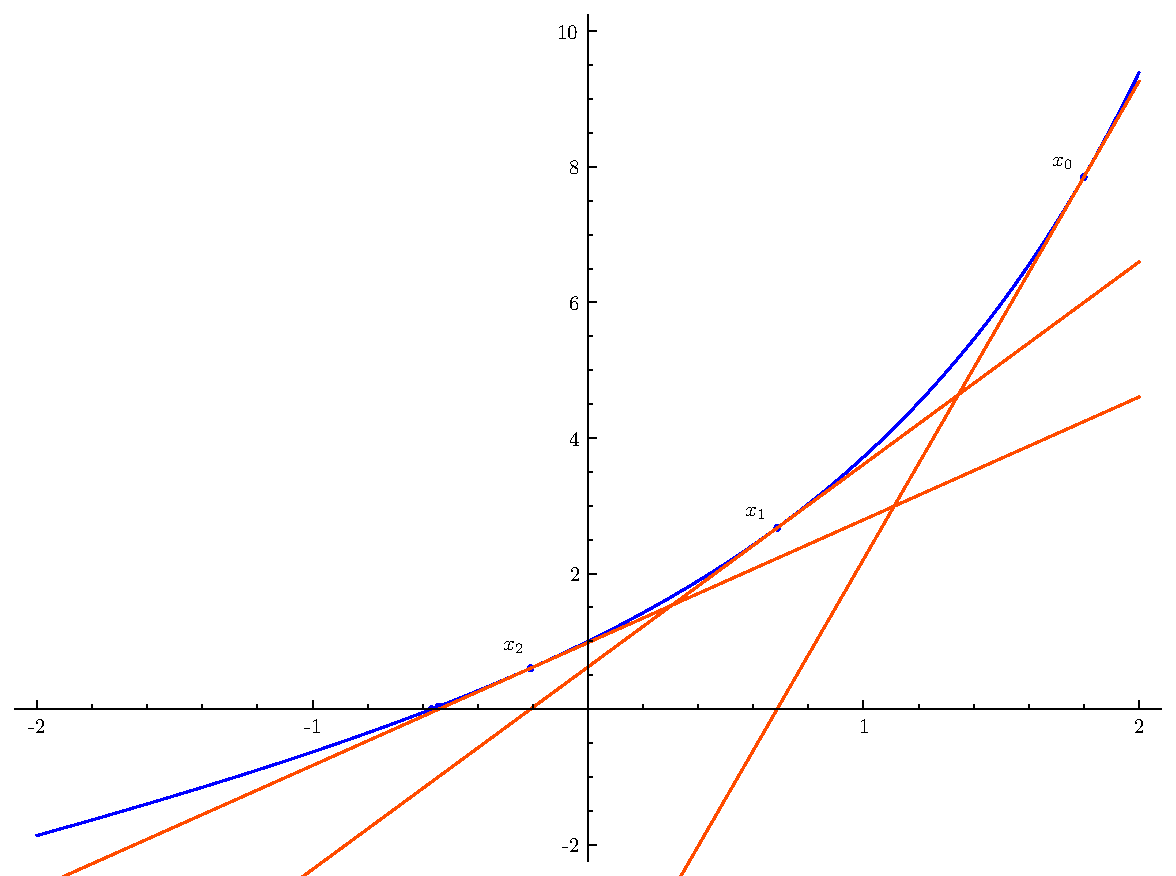
\includegraphics[width=\textwidth]{newton_iters}
\caption{An illustration of how one iteration of Newton's method works}
\end{figure}

Newton's method is powerful because of the speed of convergence.
In many cases Newton's method converges to the actual root quadratically, meaning that the error term is squared at every iteration.
This fast convergence makes it a very powerful algorithm.

Newton's method does suffer from the flaw that its convergence is dependent upon an initial guess.
If the initial guess is not sufficiently close the convergence can be much slower, or may never occur.
There are even certain pathological functions for which newton's method will never converge.
However, these functions are very rare, and as a rule Newton's method converges very quickly.



\begin{problem}
Write a Newton's method function that it runs whether or not the user inputs a derivative function.
In python this can be done by defining the derivative function as a keyword argument.
Also accept a maximum of how many iterations it will run.
Return a tuple where the first value is the value and the second value is a boolean on whether it converged or not.
Your function definition will look something like this \li{def newton(f, x0, df=None, tol=0.001, maxNum = 20000)}

Compare the performance of Newton's method when you input the derivative and when you don't.
How well does each converge?
Which runs faster?
Try the following functions:

\begin{itemize}
\item $cos(x)$
\item $x^2sin(\frac{1}{x})$
\item $(\frac{sin(x)}{x})-x$
\end{itemize}
\end{problem}

\begin{problem}
Test your newton's method function on $x^{1/3}$.
Use random starting points around zero.
What do you see?
Prove that for any non-zero starting point that newton's method will diverge.
\end{problem}

\begin{problem}
Extend your Newton's method even further so that it will work on systems of equations.
Suppose that $F: \mathbb{R}^n \rightarrow \mathbb{R}^n $.
The relevant equation is
\[
x_{i+1} = x_i - J^{-1}F(x_i)
\]
Note that you {\bf should not} calculate the inverse Jacobian.
\li{sp.solve(A,b)} gives you the solution $x$ to the equation $Ax=b$.
Use this fact to calculate $J^{-1}F$ from $J$ and $F$.
You should be able to make this function work whether or not the user inputs a Jacobian.
This also means that you will have to use your own \li{jacobian} function.
\end{problem}

\section*{Basins of Attraction and Julia Sets}
Recall Newton's method for finding the roots of a function in one variable.
Given the function $f$ and a seed value $x_0$, we can iteratively find a root:
\[
x_{n+1} = x_n - \frac{f(x_n)}{f'(x_n)}
\]
We have shown in previous sections that this method will converge very quickly to a root.
For example, given
\[
f(x) = x^2 + x -2
\]
and a seed value of $x_0 = 4$, after only 4 iterations we are about as close to the true root at $1$ as we would like.
What happens, however, when we choose a different seed value, say $x_0 = -4$?
Going through the Newton iterations, we notice that we quickly converge to the other root of the function, $-2$.

\begin{figure}
\begin{center}
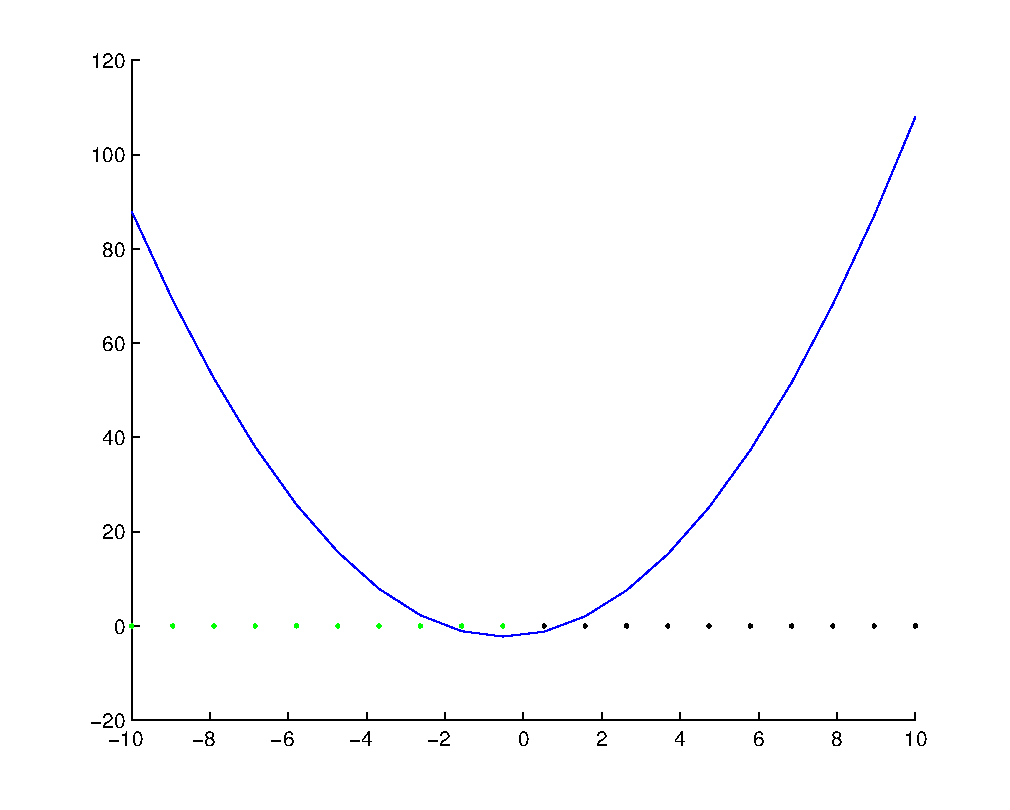
\includegraphics[scale=0.5]{basins1}
\caption{The plot of $f(x) = x^2 + x - 2$ along with 20 seed values for Newton's Method.
The green values all converge to the root at -2, and the black values will converge to the root at 1.}
\label{Fig:basins1}
\end{center}
\end{figure}

It turns out that for $f(x) = x^2 + x - 2$, any seed value will converge to one root or the other.
We call the set of points that converge to a single value through an iterative process a basin of attraction.
We can see in Figure \ref{Fig:basins1} a set of seed values that are color coded to indicate which root they converge to with Newton's method.

\begin{problem}
Write a function that will accept a function with real roots and a number of evenly spaced seed values to try.
Output an array with the starting vales as one column and the root that the converge to in the second column.
Test your function on $f(x) = x(x-1)(x+1)$.
\end{problem}

We now extend these ideas to complex functions.
There is an entire field of mathematics devoted to the study of such functions, but here we only examine some basic properties as they pertain to the generation of Julia sets.
Like other functions we have thus far been exposed to, a complex function maps an input to a unique output.
However, in this case both the input and the output come from the space of complex numbers.

Given a sufficiently ``nice'' complex function, we can apply Newton's method in a similar way to how we applied it in the real case.
However due to the nature of the space we are mapping from and to, we no longer have access to the intuitive visual representations of functions that we saw in the real case.
We can, however, graph the basins of attraction for Newton's method on the complex plane.
For example, let:
\[
f(z) = z^2 - 1
\]
Derivatives for nice complex functions behave much the same way as in the real case:
\[
f'(z) = 2z
\]
It is straightforward to verify that $f$ has two roots at 1 and -1.

In order to better visualize basins of attraction in the complex plane we will use the function li{pcolormesh} from the pyplot library in matplotlib.
The following is an example of how to use this function.
It allows us to color different portions of a plane according to the value of a function at each point.

\begin{lstlisting}
import scipy as sp
from matplotlib import pyplot as plt
n=401
x=sp.linspace(-2,2,n)
y=sp.linspace(-2,2,n)
X,Y=sp.meshgrid(x,y)
def func(x):
    return sp.real(x**3-2*x**2-x+2)
C=func(X+complex(0,1)*Y)
plt.pcolormesh(X,Y,C)
plt.show()
\end{lstlisting}

\begin{problem}
Modify your code from the previous problem to graph the basins of attraction of a function over the complex plane.
Examine the basins of attraction for the following complex functions on the following domains.
\begin{itemize}

\item $z^3 - 2 z^2 - 2 z + 2$ on the set of complex numbers $a + b i$ such that $a \in \left[-\frac{1}{2}, 0\right]$ and $b \in \left[-\frac{1}{4}, \frac{1}{4}\right]$.

\item $3 z^3 - 2 z^2 - 2 z + 2$ on the set of complex numbers $a + b i$ such that $a \in \left[-1, 1\right]$ and $b \in \left[-1, 1\right]$.

\item $z^4 + 3 z^3 - 2 z^2 - 2 z + 2$ on the set of complex numbers $a + b i$ such that $a \in \left[-1, 1\right]$ and $b \in \left[-1, 1\right]$.

\end{itemize}
Make sure that when plotting you start with low resolution.
Even if you generate a plot using an array of $100$ by $100$ points, you will be running Newton's method on your test function $10,000$ times, so be careful.  

Keeping in mind the previous problems with real valued functions, what do you expect will happen when you examine a cubic complex polynomial?
Plot the basins of attraction of $f(z) = z^3 - 1$.  What happened?
\end{problem}

The complex behavior on the boundaries of the basins of attraction of the cubic polynomial $f(z) = z^3 - 1$ is called a fractal.
This complex and beautiful behavior occurs due to a result from complex analysis that says that the basins of attraction of the Newton map must share a common boundary.
For a linear or quadratic function, this results in boring expected behavior, but when we examine a polynomial of degree 3 or higher we see the complex boundaries arise.
These complex boundaries are called the Julia set of a function (The boring parts of the picture are called the Fatou set).  
%The interested reader can find more at CITATION NEEDED. Fractal behavior lies at the heart of what is known as chaos, which will be examined in a later chapter.

To finish this section we examine the Julia sets of an iterated complex map.
In this case, instead of examining the basins of attraction of Newtons method, we will simply iterate on the complex function $f(z) = z^2 + c$ where $c \in \mathbb{C}$.
For example, let $c = 0.4 + 0.3i$ and the choose a seed value $z_0$ and iterate on $f$, i.e.
\[
f_{n+1} = f(f_n)
\]
Where $f_1 = f(z_0)$.  Try $z_0 = 0.5 + 0.1i$ and $z_0 = 5 + 5i$ as seed values.
What happens after several iterations of $f$?

\begin{figure}\label{Fig:julia}
\begin{center}
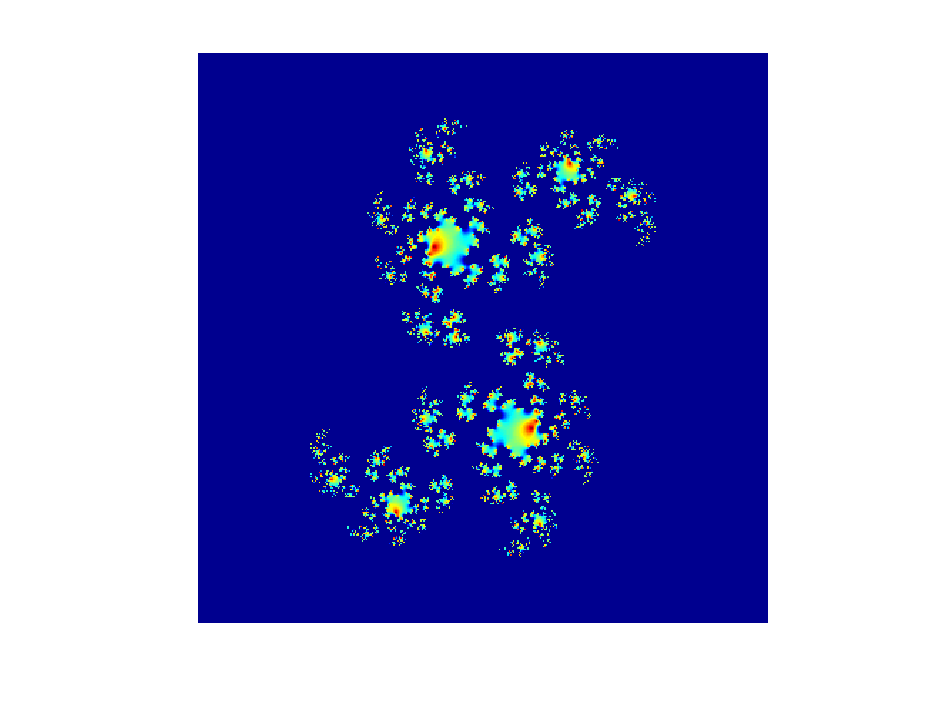
\includegraphics[scale=0.5]{julia}
\caption{We let $f(z) = z^2 + 0.4 + 0.3i$ and then iterate on a mesh from $[-1,1]\times[-i,i]$.
The above figure is a plot of $e^{-f_{30}(|z|)}$ for each $z$ in the mesh.}
\end{center}
\end{figure}

\begin{problem}
Generate another grid of complex numbers on $[-1,1]\times[-i,i]$.
Write code that iterates each point in the mesh 30 times, and then plot $e^{-f_{30}(|z|)}$ on the resulting mesh.
Try for several values of $c$.
\end{problem}
